\documentclass[12pt]{article}
\usepackage[italian]{babel}
\usepackage[dvipsnames]{xcolor}
\usepackage[utf8]{inputenc}
\usepackage{hyperref}
\usepackage{graphicx}
\usepackage{float}
\usepackage{incgraph}
\usepackage{listings} % syntax highlighting
\usepackage{tabularx}
% https://tex.stackexchange.com/a/343329/232428
\renewcommand\tabularxcolumn[1]{m{#1}}% for vertical centering text in X column


\definecolor{dkgreen}{rgb}{0,0.6,0}
\definecolor{gray}{rgb}{0.5,0.5,0.5}
\definecolor{mauve}{rgb}{0.58,0,0.82}
\definecolor{LightGray}{rgb}{0.97,0.97,0.97}

% from https://gist.github.com/vsimko/fcc84e1e4f8e750746caa34b802db5a7
\lstdefinelanguage{SPARQL}{
  basicstyle=\small\ttfamily,
  backgroundcolor=\color{LightGray},
  columns=fullflexible,
  breaklines=false,
  sensitive=true,
  numbers=left,
  % --------------------------
  frame=bt,
  aboveskip=1em,
  belowskip=1em,
  xleftmargin=.5em,
  xrightmargin=.5em,
  framexleftmargin=.5em,
  framextopmargin=.5em,
  framexbottommargin=.5em,
  framexrightmargin=.5em,
  % --------------------------
  tabsize = 2,
  showstringspaces=false,
  morecomment=[l][\color{gray}]{\#},       % comments
  morecomment=[n][\color{blue}]{<http}{>}, % uris
  morestring=[b][\color{OliveGreen}]{\"},  % strings
  % -------------------------- variables
  keywordsprefix=?,
  classoffset=0,
  keywordstyle=\color{Sepia},
  morekeywords={},
  % -------------------------- prefixes
  classoffset=1,
  keywordstyle=\color{Purple},
  morekeywords={rdf,rdfs,owl,xsd,purl},
  % -------------------------- keywords
  classoffset=2,
  keywordstyle=\color{MidnightBlue},
  morekeywords={
    SELECT,CONSTRUCT,DESCRIBE,ASK,WHERE,FROM,NAMED,PREFIX,BASE,OPTIONAL,
    FILTER,GRAPH,LIMIT,OFFSET,SERVICE,UNION,EXISTS,NOT,BINDINGS,MINUS,a
  }
}


\newcommand\blankpage{
    \null
    \thispagestyle{empty}
    \newpage
    }

\begin{document}

\begin{titlepage}

\thispagestyle{empty}

\centerline {\Large{\MakeUppercase{ Università DEGLI STUDI DI TORINO}}}
\vskip 20 pt

\centerline {\Large{\textsc DIPARTIMENTO DI INFORMATICA}}

\vskip 20 pt

\centerline {{\textsc SCUOLA DI SCIENZE DELLA NATURA}}

\vskip 20 pt

\centerline {\Large{\textsc Corso di Laurea Magistrale in Informatica}}

\vskip 50 pt


%\begin{tabular}{ccc}
\centerline {\includegraphics[width=4cm]{files/Unito-logo.png}}
%   \end{tabular}

\vskip 2cm

\centerline {\Large {\bf Progetto Modellazione Concettuale del Web Semantico}}

\vskip 1.7cm

\noindent Lorenzo \textsc{Sciandra}
\hfill  {Stefano Vittorio \textsc{Porta}}



\vskip 2.7cm


\centerline{ANNO ACCADEMICO}
\vskip 0.1cm
\centerline{2020/2021}

\end{titlepage}

\section{Pagina del progetto}
Tutto quello che sarà presentato in questa documentazione può essere facilmente esplorato mediante il link pubblico del \href{https://github.com/LorenzoSciandra/ProgettoModSem}{repository Github} o attraverso la sua \href{https://lorenzosciandra.github.io/ProgettoModSem/}{pagina HTML}.  

\section{Motivazioni}
Il dominio che abbiamo deciso di modellare riguarda il campo della ristorazione. 
Durante l'analisi abbiamo prestato particolare attenzione alla gestione di alcuni aspetti che abbiamo ritenuto particolarmente importanti:
\begin{itemize}
    \item Gli Esercizi alimentari (Ristoranti, Bar, Paninoteche, ecc);
    \item Le Pietanze servite dagli esercizi alimentari e gli Ingredienti che le compongono;
    \item Le varie Attività collegate agli Esercizi alimentari ed effettuate da Persone, come Ordini, Consegne, Recensione e Amministrazione.
\end{itemize}
L'idea è nata pensando all'offerta sempre più diffusa dei servizi di consegna a domicilio.
Infatti, date le restrizioni sanitarie vigenti, un numero in costante aumento di imprese di ristorazione sta ricorrendo a servizi di consegne a domicilio, non solo nelle grandi città, ma anche in centri urbani di più modeste dimensioni\footnote{\url{https://www.ilsole24ore.com/art/coronavirus-e-boom-spesa-online-consegna-domicilio-AD3rKdC}} \footnote{\url{https://www.repubblica.it/economia/rapporti/osserva-italia/trend/2020/10/16/news/cresce_la_passione_per_il_cibo_a_domicilio-270779771/}}.\newline
Esistono svariati servizi (alcuni dei quali molto rinomati e popolari) che fungono da mediatore tra la proposta dei locali e la richiesta dei clienti. 
Tuttavia, nessuno sembra fare affidamento ad una gestione semantica dei propri dati, preferendo piuttosto dei sistemi più standard.\newline
L'idea di creare un'ontologia comune che modelli correttamente questo dominio potrebbe quindi risultare utile per offrire uno strumento particolare e potente, in grado di facilitare la gestione per tutte le parti e migliorare le possibili applicazioni.\newline
Un secondo punto cruciale riguarda gli allergeni: tra le varie piattaforme di delivery esistenti da noi provate, nessuna permette di filtrare i locali con la precisione che pensavamo di offrire (in funzione degli allergeni presenti nelle pietanze proposte\footnote{Si veda ad esempio Just Eat: \url{https://www.justeat.it/help/article/115001318051/cosa-faccio-se-sono-allergico-a-qualcosa}} o dell'alimentazione corrispondente).
Questi criteri di ricerca sono stati da noi tenuti in considerazione durante la modellazione.

\section{Requisiti}

\subsection{Finalità}
Lo scopo dell'ontologia riguarda un'ipotetica piattaforma di delivery che possa permettere a dei locali di esporsi facilmente con le proprie proposte a un insieme di utenti a cui intendono rivolgersi per saziare le proprie esigenze alimentari. 
Il tutto attraverso una struttura su cui sia facile effettuare reasoning, per  inferire pietanze incompatibili o meno con diete (veganismo, vegetarianismo) o con intolleranze ed allergie (come la celiachia, l'intolleranza al lattosio o il favismo).\newline 
Con l'ontologia, una volta effettuato reasoning, gli utenti potranno quindi filtrare i piatti non solo in base alla città o alla tipologia di locale, ma anche a seconda della presenza o meno di piatti conformi a diete e disturbi o facendo riferimento a precedenti recensioni.\newline
La nostra intenzione è di sfruttare il più possibile le potenzialità del reasoning, in modo da ridurre al minimo indispensabile il tempo e i dati necessari da introdurre manualmente per il funzionamento dell'ontologia.\newline
Seguono due mockup dell'ipotetica piattaforma di delivery immaginata:
\label{sec:mockupFinali}
\begin{figure}[H]
    \centering
         \includegraphics[width=12cm]{files/mockup1.jpg}
    \caption{Pagina iniziale di ricerca}
\end{figure}
\begin{figure}[H]
    \centering
         \includegraphics[width=12cm]{files/mockup2.jpeg}
    \caption{Risultati della ricerca di locali a Torino}
\end{figure}

\subsection{Task specifici e contesto}
I task principali che l'ontologia punta a rendere effettuabili sono:
\begin{itemize}
    \item Ricerca di locali in una certa città, utilizzando filtri per i generi di pietanze servite e per gli allergeni;
    \item Gestione di un locale e delle pietanze servite;
    \item Introduzione e modifica di ingredienti e pietanze, indicabili come offerte da più locali;
    \item Pubblicazione di recensioni dei locali;
    \item Gestione delle attività di ordine e consegna da parte di addetti e proprietari delle attività.
\end{itemize}

\subsection{Utenti target}
\begin{itemize}
    \item \textbf{Proprietari di esercizi alimentari} che vogliono gestire il traffico lavorativo del loro locale;
    \item \textbf{Persone che lavorano nel settore delle consegne} e che usano l'applicativo per trovare nuovi ordini da recapitare;
    \item \textbf{Clienti} che vogliono effettuare un ordine da un locale o recensire un posto dopo una consumazione.
\end{itemize}

\section{Descrizione del Dominio e Fonti}
\subsection{Dominio}
Il dominio, collocato nell'ambito dei servizi di consegna, ha come fine la rappresentazione di Locali, Pietanze, Ingredienti, Disturbi alimentari e Persone.\newline
Queste cinque classi principali sono correlate tra di loro:
\begin{itemize}
    \item Le pietanze sono composte da vari ingredienti, oppure ne utilizzano alcuni come mezzo per la cottura (ad esempio frittura). Inoltre ereditano dagli ingredienti che le compongono le \textbf{incompatibilità} con gli stessi disturbi alimentari;
    \item Gli ingredienti possono essere composti a loro volta da altri ingredienti, e in questo modo è possibile descrivere precisamente la composizione delle pietanze. In modo simile alle pietanze, anche gli ingredienti ereditano dagli ingredienti di cui sono composti le \textbf{incompatibilità} con i disturbi alimentari indicati o inferiti;
    \item Multipli Locali possono servire le stesse pietanze. Inoltre, le Persone possono piazzare ordini (consegnati da altre Persone), pubblicare recensioni riguardo un certo ordine e aprire nuovi Locali.
\end{itemize}
\subsection{Fonti}
In modo da poter rappresentare adeguatamente il dominio, ci siamo basati prevalentemente su siti web.\newline
Per gli allergeni, abbiamo fatto affidamento a:
\begin{itemize}
    \item "\href{https://it.wikipedia.org/wiki/Allergeni_alimentari}{Allergeni alimentari}", su \textit{Wikipedia};
    \item "\href{https://it.wikipedia.org/wiki/Carenza_di_glucosio-6-fosfato_deidrogenasi}{Carenza di glucosio-6-fosfato deidrogenasi (Favismo)}", su \textit{Wikipedia};
    \item "\href{https://it.wikipedia.org/wiki/Intolleranza_al_lattosio}{Intolleranza al Lattosio}", su \textit{Wikipedia};
    \item "\href{https://www.celiachia.it/}{Celiachia}", sul sito dell'\textit{Associazione Italiana Celiachia};
    \item "\href{http://www.ospedalebambinogesu.it/allergia-alla-frutta-a-guscio}{Allergia alla frutta a guscio}", sul sito dell'\textit{Ospedale Bambino Gesù};
    \item "\href{https://www.orpha.net/consor/cgi-bin/OC_Exp.php?lng=it&Expert=469}{Intolleranza al Fruttosio}" sul \textit{Portale delle malattie rare e dei farmaci orfani};
    \item "\href{https://www.fondazioneveronesi.it/magazine/articoli/lesperto-risponde/allergia-al-nichel-quali-precauzioni-prendere-cucina}{Allergia al Nickel}", sul sito della \textit{Fondazione Veronesi}.
\end{itemize}
Per le informazioni sulle consegne abbiamo fatto affidamento ad alcuni siti che offrono servizi di delivery (\href{https://www.justeat.it/}{Just Eat}, \href{https://glovoapp.com}{Glovo}, \href{https://deliveroo.it}{Deliveroo}).\newline
Le informazioni sulle città provengono da \href{https://it.wikipedia.org/}{Wikipedia} e \href{https://www.google.it/maps}{Google Maps}.\newline
Infine per le Pietanze abbiamo utilizzato le ricette di \href{https://www.giallozafferano.it/}{Giallo Zafferano}, di alcuni libri di cucina in nostro possesso (tra cui "\href{https://www.anobii.com/books/Muffin_scone_e_torte/9788880584278/01119011f24adbf79a}{Muffin, Scone e Torte}") e alcune preparazioni che conosciamo e prepariamo in casa.

\newpage
\section{Documentazione del Dominio}
\subsection{Risorse simili ed ispirazione}
La nostra ontologia spazia su un buon numero di tematiche; possiamo affermare che le ispirazioni e le risorse utilizzate siano piuttosto variegate.
\newline
Cominciamo mostrando siti noti che offrono servizi di delivery, da cui abbiamo in parte tratto ispirazione. Iniziamo dalla schermata di ricerca di Just Eat una volta selezionata \textit{Via Pessinetto 12}, a Torino:
\begin{figure}[H]
    \centering
    \includegraphics[width=12cm]{files/justEat.png}
    \caption{Alcuni locali elencati su Just Eat nelle vicinanze del Dipartimento}
\end{figure}
Come è possibile notare, i filtri che un utente può applicare si allontanano da quelle che sono le nostre idee. I locali vengono infatti filtrati solamente in base al tipo di cucina che offrono, alle stelle associate e alla presenza o meno della consegna gratuita. Non vi è alcun tipo di riferimento a diete o allergie.\newline
Spostiamoci ora su Glovo che sembra avvicinarsi di più alle nostre intenzioni:
\begin{figure}[H]
    \centering
    \includegraphics[width=12cm]{files/glovo.png}
    \caption{Alcuni locali registrati per il comune di Torino}
\end{figure}
\`{E} possibile notare come Glovo presenti alcune delle nostre idee.\newline
In primo luogo è data la possibilità di filtrare i locali in base alla città senza essere costretti, a differenza di Just Eat, a specificare un indirizzo in particolare. In secondo luogo, è possibile filtrare i ristoranti in una città anche in base alla dieta (è disponibile tuttavia solo quella Vegetariana) e all'attributo "senza glutine". Manca però in questo caso la possibilità di filtrare i locali in base alle valutazioni degli utenti e la scelta delle diete/allergie come criteri sono molto scarsi. \newline
La piattaforma da noi immaginata presenta il meglio dei criteri di questi due siti, ampliandoli: la possibilità di scremare i risultati in base ad un ricco catalogo di allergie e diete senza però trascurare l'importanza delle recensioni dei clienti che avvalorano o meno un locale.
\par 
Cambiamo ora completamente tipologia di risorsa per analizzare un altro aspetto di Delivery Doctor: la tassonomia che descrive le pietanze e gli ingredienti che le compongono. Non possiamo non citare in questo caso Giallo Zafferano:
\begin{figure}[H]
    \centering
    \includegraphics[width=13cm]{files/GialloZafferano.jpg}
    \caption{Una ricetta per la Pizza Margherita descritta da Giallo Zafferano}
\end{figure}
Come si può vedere nell'immagine precedente, una pietanza come la pizza margherita (presente anche nella nostra ontologia) viene descritta con moltissimi dettagli: non sono presenti solo gli ingredienti necessari (che ci permettono di classificarla come pietanza vegetariana) ma anche tempi di cottura/preparazione, calorie e tutte le fasi della preparazione, con l'aggiunta di immagini e contenuti video.\newline
Da qui deriva la nostra idea di arricchire le pietanze proposte dai vari esercizi alimentari con gli ingredienti che le compongono. In questo modo anche la nostra ontologia è in grado di inferire la compatibilità o meno di un piatto con diete o disturbi alimetari, e come conseguenza è possibile per l'utente filtrare i locali in maniera coerente con le sue esigenze.
\par
Per quanto riguarda invece la classificazione dei disturbi alimentari ci siamo ispirati alla decima versione del thesauro \href{https://bioportal.bioontology.org/ontologies/ICD10CM}{"\textit{International Classification of Diseases}"} dell'OMS, al quale ci siamo anche allineati:
\begin{figure}[H]
    \centering
    \includegraphics[width=13cm]{files/thesauroBio.png}
    \caption{Descrizione della celiachia nell'ICD10.}
\end{figure}

% Spiegazione dell'ispirazione 
% Screenshot e qualche spiegzione sui siti di delivery, ricette; per gli allergeni vari siti o bibliografia

\subsection{Allineamenti}
Oltre all'allineamento con con l'\textit{International Classification of Diseases}, già presentato nella sezione precedente, ci siamo allineati con \href{https://schema.org/}{Schema.org}, da noi usato per la  localizzazione geografica dei locali e per i concetti inerenti la recensione degli stessi.\newline
Per quanto riguarda la modellazione delle azioni abbiamo fatto riferimento a \href{https://www.w3.org/TR/prov-o/}{Provenance} e in particolare il PROV Model, dal quale abbiamo definito delle sottoclassi più specifiche e delle sottoproprietà che collegassero le nuovi classi.
\begin{figure}[H]
    \centering
    \includegraphics[width=10cm]{files/provenacePattern.png}
    \caption{\href{https://en.wikipedia.org/wiki/PROV_(Provenance)}{PROV Model}}
\end{figure}
A partire dalle classi \textbf{Activity, Entity, Agent} e \textbf{Role} abbiamo introdotto le azioni \textit{Recensire, Ordinare, Consegnare} e \textit{Avviare Impresa} ponendole come \texttt{rdfs:subClassOf} \texttt{prov:Activity}. Attorno all'attività ruotano i concetti di:
\begin{itemize}
    \item \textbf{Agente}, colui che fa l'azione;
    \item \textbf{Ruolo}, il compito svolto dalla persona nell'\texttt{Activity} ed entità che identifica elementi creati o usati nel corso dell'azione.
\end{itemize}

\section{LODE}
Al momento della progettazione di Delivery Doctor, il progetto \href{https://github.com/essepuntato/LODE}{LODE} sviluppato da Silvio Peroni presenta alcuni problemi tecnici, e spesso il servizio online è irraggiungibile. Per poter ottenere una documentazione completa dell'ontologia è stato quindi utilizzata un'alternativa che imita in tutto e per tutto LODE: \href{https://github.com/RDFLib/pyLODE}{pyLODE}. Si tratta di un'implementazione in python, utilizzabile in locale.\newline
Una copia aggiornata della documentazione è disponibile sul \href{https://lorenzosciandra.github.io/ProgettoModSem/documentazione/lode.html}{repository github dell'Ontologia}.

%aggiungere un href al repo

\section{Visualizzazione Ontologia}
    Vediamo ora una versione grafica dell'ontologia che ne espliciti le relazioni tra le varie classi mediante sussunzione.
    \begin{figure}[H]
        \makebox[\textwidth][c]{\includegraphics[width=18cm]{files/gerarchia.png}}
        \caption{Gerarchia delle classi}
    \end{figure}
    Come si evince dalla tassonomia appena presentata, a cui si rimanda all'ultima sezione per una visione ingrandita, per quanto riguarda la modellazione delle pietanze come insieme di ingredienti che le compongono abbiamo usato l' \href{http://ontologydesignpatterns.org/wiki/Submissions:Set}{Ontology Design Pattern Set}:
    \begin{figure}[H]
        \centering
          \includegraphics[width=12cm]{files/ODPSet.png}
        \caption{ODP Set}
    \end{figure}
    Abbiamo quindi definito la Pietanza come sussunta a Set ed usato la object property ereditata "hasMember" per la definizione delle nuove proprietà "utilizza ingrediente" e "utilizza indirettamente l'ingrediente" che collegano direttamente la pietanza con gli ingredienti di cui è composta.
    \newline
    Mostriamo ora due esempi tratti da Graph DB composti da un insieme di triple e dal Visual graph ad esse associato.
    \newline
    Partiamo dall'ordine effettuato da un utente generico Luca presso il Dubai Coffee Lounge:
    \begin{figure}[H]
        \makebox[\textwidth][c]{\includegraphics[width=20cm]{files/lucaOrderTriple.png}}
        \caption{Insieme delle triple usate per modellare l'ordine di Luca}
    \end{figure}
    \newpage
    Una visualizzazione grafica di questo è la seguente:
    \begin{figure}[H]
        \makebox[\textwidth][c]{\includegraphics[width=15cm]{files/esempioOrdineLuca.png}}
        \caption{Visual Graph associato all'ordine di Luca}
    \end{figure}
    Come altro esempio presenteremo la modellazione dell'entità Pizza Margherita collegandoci con quanto presentato nella sezione 5 e la sua definizione in Giallo Zafferano.
    \newline
    Iniziamo mostrando le triple ad essa collegate:
    \begin{figure}[H]
        \makebox[\textwidth][c]{\includegraphics[width=20cm]{files/pizzaTriple.png}}
        \caption{Insieme delle triple usate per modellare la pizza margherita}
    \end{figure}
    Mostriamo ora, esattamente come prima, la loro trasposizione grafica:
    \begin{figure}[H]
        \makebox[\textwidth][c]{\includegraphics[width=15cm]{files/pizzaGrafo.png}}
        \caption{Visual Graph associato alla pizza margherita}
    \end{figure}
\section{Ontologia in formato Turtle}
Per visionare l'ontologia in formato Turtle rimandiamo il lettore alla \href{https://lorenzosciandra.github.io/ProgettoModSem/}{pagina del progetto}.

\section{Queries SPARQL}
Suddivideremo questa sezione in 4 parti: la prima contenente l'interazione e quindi le queries di un untente normale, la seconda per l'utente proprietario di un esercizio alimentare, la terza riguardano invece l'interazione di un fattorino e l'ultima parte sarà dedicata alle queries dirette verso risorse ontologiche esterne.

\subsection{Utente Normale}
Il flusso d'interazione dell'utente generico Luca riguarderà l'iniziale ricerca dei locali nella sua città, Torino, per poi filtrare i risultati sulla base degli esercizi alimentari che dispongono di almeno una pietanza compatibile con la celiachia. Terminerà l'interazione visionando tutti gli ordini compiuti.
\begin{figure}[H]
    \centering
         \includegraphics[width=9cm]{files/lucaInterazione.png}
    \caption{Interazione tra Luca e la piattaforma}
\end{figure}

Iniziamo con la Query che permette all'utente di ottenere tutti i locali situati a Torino.
\begin{lstlisting}[language=SPARQL]
PREFIX rdf: <http://www.w3.org/1999/02/22-rdf-syntax-ns#>
PREFIX deliverydr: 
<http://www.semanticweb.org/progettomodsem2020/deliverydoctor#>
    
SELECT ?localeNome WHERE{
    ?locale deliverydr:localeSituatoInCitta ?citta;
        deliverydr:haNome ?localeNome.
    ?citta deliverydr:haNome "Torino".
}
\end{lstlisting}
Con risultato:
\newline
\newline
\begin{tabularx}{\textwidth} { 
  | >{\centering\arraybackslash}X |}
 \hline
 \textbf{?localeNome} \\
 \hline
 \textit{Dubai Coffee Lounge}\\
 \hline
 \textit{Napples}\\
\hline
\end{tabularx}
\newline
\newline
L'utente ora filtrerà i risultati ottenuti cercando i locali e le rispettive pietanze servite compatibili con il disturbo celiachia.
\begin{lstlisting}[language=SPARQL]
PREFIX rdf: <http://www.w3.org/1999/02/22-rdf-syntax-ns#>
PREFIX deliverydr:
<http://www.semanticweb.org/progettomodsem2020/deliverydoctor#>
    
SELECT ?localeNome ?pietanza WHERE {
    ?locale deliverydr:localeSituatoInCitta ?citta;
        deliverydr:localeServePietanza ?pietanza;
        deliverydr:haNome ?localeNome.
    ?pietanza deliverydr:pietanzaCompatibileConDisturbo 
                                        deliverydr:Celiachia,
                                        deliverydr:AllergiaGlutine.
    ?citta deliverydr:haNome "Torino".
}
\end{lstlisting}
Ottenendo come risultato:
\newline
\newline
\begin{tabularx}{\textwidth} { 
  | >{\centering\arraybackslash}X 
  | >{\centering\arraybackslash}X |}
 \hline
 \textbf{?localeNome} & \textbf{?pietanza} \\
 \hline
 \textit{Dubai Coffee Lounge} & \textit{deliverydr:CappuccinoSpeciale}  \\
 \hline
 \textit{Dubai Coffee Lounge} & \textit{deliverydr:RisottoSugo}\\
\hline
\end{tabularx}
\newline
\newline
Come possiamo notare dall'insieme dei locali verrà escluso Napples che nella nostra ontologia propone solo pizze e in maniera analoga tra le pietanze proposte dal Dubai verranno filtrate solo quelle compatibili con la celiachia/allergia al glutine.
\newline
Supponiamo ora che il nostro utente Luca voglia vedere lo storico degli ordini che ha effettuato.
\begin{lstlisting}[language=SPARQL]
PREFIX rdf: <http://www.w3.org/1999/02/22-rdf-syntax-ns#>
PREFIX deliverydr:
<http://www.semanticweb.org/progettomodsem2020/deliverydoctor#>

SELECT ?ordine ?localeNome ?pietanza WHERE{
    ?ordinare deliverydr:ordinatoDa ?persona;
        deliverydr:ordinareDalLocale ?locale.
    ?ordine deliverydr:ordineCreatoDaAzione ?ordinare;
        deliverydr:ordineCompostoDaPietanza ?pietanza.
    ?locale deliverydr:haNome ?localeNome.
    ?persona deliverydr:haNome "Luca".
}
\end{lstlisting}
\begin{tabularx}{\textwidth} { 
  | >{\centering\arraybackslash}X 
  | >{\centering\arraybackslash}X
  | >{\centering\arraybackslash}X |}
 \hline
 \textbf{?ordine} & \textbf{?locale} & \textbf{?pietanza} \\
 \hline
 \textit{deliverydr: CappuccinoECroissant} & \textit{Dubai Coffee Lounge} & \textit{deliverydr: CappuccinoSpeciale}  \\
 \hline
 \textit{deliverydr: CappuccinoECroissant} & \textit{Dubai Coffee Lounge} & \textit{deliverydr:Croissant}\\
\hline
\end{tabularx}

\subsection{Utente Proprietario}
Nel caso dell'Utente Proprietario, il flusso d'interazione è più frammentato, dato che i compiti che deve assolvere sono molteplici, e come esempio può:
\begin{enumerate}
    \item Controllare gli ordini che la sua attività ha ricevuto
    \item Controllare le recensioni lasciate dagli utenti sulla sua attività
    \item Visionare il menù proposto dall'attività per valutare eventuali cambiamenti
\end{enumerate}
Supponendo che il Proprietario diriga il locale "Dubai Coffee Lounge", è piuttosto immediata la ricerca di tutti gli ordini che gestisce e delle pietanze richieste:
\begin{figure}[H]
    \centering
         \includegraphics[width=8cm]{files/Proprietario 1.png}
    \caption{Il Proprietario richiede gli ordini gestiti per uno specifico locale}
\end{figure}
\begin{lstlisting}[language=SPARQL]
PREFIX rdf: <http://www.w3.org/1999/02/22-rdf-syntax-ns#>
PREFIX rdfs: <http://www.w3.org/2000/01/rdf-schema#>
PREFIX deliverydr:
<http://www.semanticweb.org/progettomodsem2020/deliverydoctor#>

SELECT ?ordine ?persona ?pietanza WHERE {
    ?locale deliverydr:haNome "Dubai Coffee Lounge".
    ?ordine deliverydr:ordineCompostoDaPietanza ?pietanza;
             deliverydr:ordineCreatoDaAzione ?azione.
    ?azione deliverydr:ordinatoDa ?persona;
             deliverydr:ordinareDalLocale ?locale.
}
\end{lstlisting}
\begin{tabularx}{\textwidth} {
  | >{\centering\arraybackslash}X 
  | >{\centering\arraybackslash}X
  | >{\centering\arraybackslash}X |}
 \hline
 \textbf{?ordine} & \textbf{?persona} & \textbf{?pietanza} \\
 \hline
 \textit{deliverydr: CappuccinoECroissant} & \textit{deliverydr:Luca} & \textit{deliverydr:Croissant} \\
 \hline
 \textit{deliverydr: CappuccinoECroissant} & \textit{deliverydr:Luca} & \textit{deliverydr: CappuccinoSpeciale}  \\
 \hline
\end{tabularx}
\newline
\newline
\newline
Assieme alla visualizzazione degli ordini gestiti, potrebbe essere utile sapere cosa pensano i clienti del locale e del servizio che offre. Per far ciò, è necessario recuperare alcuni dati:
\begin{figure}[H]
    \centering
         \includegraphics[width=8cm]{files/Proprietario 2.png}
    \caption{Il Proprietario richiede le recensioni pubblicate per uno specifico locale}
\end{figure}
\begin{lstlisting}[language=SPARQL]
PREFIX rdfs: <http://www.w3.org/2000/01/rdf-schema#>
PREFIX schema: <http://schema.org/>
PREFIX deliverydr: 
<http://www.semanticweb.org/progettomodsem2020/deliverydoctor#>

SELECT ?persona ?testo ?stelle WHERE {
    ?locale deliverydr:haNome "Dubai Coffee Lounge".
    ?azione deliverydr:recensireLocale ?locale;
    	deliverydr:recensitoDa ?persona;
    	deliverydr:scrivereRecensione ?recensione.
    ?recensione schema:reviewBody ?testo;
                 schema:reviewRating ?rating.
    ?rating deliverydr:possiedeStelle ?stelle
}
\end{lstlisting}
\begin{tabularx}{\textwidth} {
  | >{\centering\arraybackslash}X 
  | >{\centering\arraybackslash}X
  | >{\centering\arraybackslash}X |}
 \hline
 \textbf{?persona} & \textbf{?testo} & \textbf{?stelle} \\
 \hline
 \textit{deliverydr:Luca} & \textit{Servono un'ottima cheesecake e dei...} & \textit{5}  \\
 \hline
\end{tabularx}
\newline
\newline
\newline
Infine, se volesse vedere le pietanze che il locale serve al momento, per variare il menù (tenendo conto del numero di ingredienti che le compongono):
\begin{figure}[H]
    \centering
         \includegraphics[width=8cm]{files/Proprietario 3.png}
    \caption{Il Proprietario richiede le pietanze servite in uno specifico locale, richiedendo successivamente anche il numero complessivo di ingredienti utilizzati}
\end{figure}
\begin{lstlisting}[language=SPARQL]
PREFIX rdfs: <http://www.w3.org/2000/01/rdf-schema#>
PREFIX deliverydr: 
<http://www.semanticweb.org/progettomodsem2020/deliverydoctor#>

SELECT ?pietanza 
(count(DISTINCT ?ingrediente) AS ?numero_ingredienti) 
WHERE {
    ?locale deliverydr:haNome "Dubai Coffee Lounge".
    ?locale deliverydr:localeServePietanza ?pietanza.
    ?pietanza deliverydr:utilizzaIngrediente ?ingrediente.
}
GROUP BY ?pietanza
\end{lstlisting}
\begin{tabularx}{\textwidth} { 
  | >{\centering\arraybackslash}X 
  | >{\centering\arraybackslash}X |}
 \hline
 \textbf{?pietanza} & \textbf{?numero\_ingredienti} \\
 \hline
 \textit{deliverydr:PolpetteAlSugo} & \textit{3}  \\
 \hline
 \textit{deliverydr:CappuccinoSpeciale} & \textit{2}  \\
 \hline
 \textit{deliverydr:LasagneAlForno} & \textit{6}  \\
 \hline
 \textit{deliverydr:Croissant} & \textit{4}  \\
 \hline
 \textit{deliverydr:RisottoSugo} & \textit{2}  \\
 \hline
\end{tabularx}
\newline
\newline
\newline
Potrebbe essere utile conoscere anche il numero di ingredienti non direttamente utilizzati dalla pietanza. In tal caso la query richiede anche una UNION:
\begin{lstlisting}[language=SPARQL]
PREFIX rdfs: <http://www.w3.org/2000/01/rdf-schema#>
PREFIX deliverydr: 
<http://www.semanticweb.org/progettomodsem2020/deliverydoctor#>

SELECT ?pietanza 
(count(DISTINCT ?ingrediente) AS ?numero_ingredienti) 
WHERE {
    ?locale deliverydr:haNome "Dubai Coffee Lounge".
    ?locale deliverydr:localeServePietanza ?pietanza.
    {?pietanza deliverydr:utilizzaIngrediente ?ingrediente}
     UNION 
    {?pietanza deliverydr:utilizzaIngredienteIndirettamente 
        ?ingrediente}
}
GROUP BY ?pietanza
\end{lstlisting}
In questo caso i valori contenuti nella colonna del numero di ingredienti saranno leggermente differenti:
\newline
\newline
\begin{tabularx}{\textwidth} { 
  | >{\centering\arraybackslash}X 
  | >{\centering\arraybackslash}X |}
 \hline
 \textbf{?pietanza} & \textbf{?numero\_ingredienti} \\
 \hline
 \textit{deliverydr:PolpetteAlSugo} & \textit{14}  \\
 \hline
 \textit{deliverydr:CappuccinoSpeciale} & \textit{4}  \\
 \hline
 \textit{deliverydr:LasagneAlForno} & \textit{15}  \\
 \hline
 \textit{deliverydr:Croissant} & \textit{6}  \\
 \hline
 \textit{deliverydr:RisottoSugo} & \textit{3}  \\
 \hline
\end{tabularx}

\subsection{Utente Fattorino}
Per l'interazione con l'utente adibito alle consegne degli ordini, vediamo una tipica azione che potrebbe fare il fattorino Gianni, come controllare tutte le consegne che ha portato a termine.

\begin{figure}[H]
    \centering
         \includegraphics[width=8cm]{files/interazioneGianni.png}
    \caption{Interazione tra Gianni e la piattaforma}
\end{figure}

\begin{lstlisting}[language=SPARQL]
PREFIX rdf: <http://www.w3.org/1999/02/22-rdf-syntax-ns#>
PREFIX deliverydr:
<http://www.semanticweb.org/progettomodsem2020/deliverydoctor#>

SELECT ?consegna ?ordine ?localeNome ?destinatario WHERE{
    ?consegna deliverydr:consegnareAlCliente ?destinatario;
        deliverydr:consegnatoDa ?persona;
        deliverydr:consegnareOrdine ?ordine.
    ?ordine deliverydr:ordineCreatoDaAzione ?ordinare.
    ?ordinare deliverydr:ordinareDalLocale ?locale.
    ?locale deliverydr:haNome ?localeNome.
    ?persona deliverydr:haNome "Gianni".
}
\end{lstlisting}
\begin{tabularx}{\textwidth} { 
  | >{\centering\arraybackslash}X 
  | >{\centering\arraybackslash}X
  | >{\centering\arraybackslash}X
  | >{\centering\arraybackslash}X |}
 \hline
 \textbf{?consegna} & \textbf{?ordine} & \textbf{?localeNome} & \textbf{destinatario} \\
 \hline
 \textit{deliverydr:} & \textit{deliverydr:} & \textit{deliverydr:} & \textit{deliverydr:}  \\
 \textit{ConsegnaOrdine} & \textit{CappuccinoE}& \textit{Dubai} & \textit{Luca}\\
 \textit{Luca} & \textit{Croissant} & \textit{Coffee Lounge}& \\
\hline
\end{tabularx}
\newline
\newline

\subsection{Queries verso risorse esterne}
Verrà prima presentata un flowchart dell'interazione per poi soffermarci sulle due queries.

\begin{figure}[H]
    \centering
         \includegraphics[width=11cm]{files/interazioneEsterna.png}
    \caption{Schema interazione utente-piattaforma-wikidata}
\end{figure}
Come primo esempio di query indirizzata verso risorse esterne supponiamo la situazione in cui un utente, dopo aver visto gli ingredienti che compongono una pietanza, sia interessato ad ottenere informazioni su uno di essi.
\newline
Supponiamo ad esempio che un utente, osservi le lasagne servite dal \textit{Dubai Coffee Lounge} e voglia avere più informazioni riguardo la besciamella che le compone:
\begin{lstlisting}[language=SPARQL]
PREFIX skos: <http://www.w3.org/2004/02/skos/core#>
PREFIX rdfs: <http://www.w3.org/2000/01/rdf-schema#>
PREFIX schema: <http://schema.org/>
PREFIX deliverydr: 
<http://www.semanticweb.org/progettomodsem2020/deliverydoctor#>

SELECT ?immagine ?descrizioneBase ?informazioneExtra
WHERE {
    ?ingr skos:prefLabel "${this.secondSelection}"@it;
          rdfs:comment ?descrizioneBase.

    FILTER ( lang(?descrizioneBase) = "it" ).
    
    OPTIONAL {
        ?ingr deliverydr:entitaWikidata ?entita.
    
        SERVICE <https://query.wikidata.org/sparql> {
            OPTIONAL {
                ?entita <http://www.wikidata.org/prop/direct/P18>
                                                                ?img.
            }
            OPTIONAL {
                ?entita schema:description ?info.
            }
        }
    
        FILTER ( lang(?informazioneExtra) = "it")
    
        BIND(COALESCE(?img, "n/a") AS ?immagine).
        BIND(COALESCE(?info, "n/a") AS ?informazioneExtra).
    }
}

LIMIT 1
\end{lstlisting}
Come risultato otteniamo l'immagine di Wikidata della besciamella, assieme alla descrizione base presente nell'ontologia e la descrizione dell'ingrediente estratta sempre da wikidata.
\newline
\newline
\begin{tabularx}{\textwidth} { 
  | >{\centering\arraybackslash}X
  | >{\centering\arraybackslash}X
  | >{\centering\arraybackslash}X |}
 \hline
 \textbf{?immagine} & \textbf{?descrizioneBase} & \textbf{?informazioneExtra} \\
 \hline
 \textit{https://upload.wikimed} \textit{ia.org/wikipedia/...} & \textit{Salsa base della cucina italiana, composta da farina, burro, latte e aromatizzata con noce moscata} & \textit{salsa di base utilizzata per ricette più complesse} \\
\hline
\end{tabularx}
\newline
\begin{figure}[H]
    \centering
         \includegraphics[width=7cm]{files/Lasagne_al_forno_salsa_besciamella.jpg}
    \caption{Immagine referenziata dal link ricevuto}
\end{figure}
Come secondo caso immaginiamo invece un utente straniero in visita alla città di Torino.\newline
Volendo trovare dei locali presso i quali poter ordinare, potrebbe essere interessato ad ottenere una mappa della città su cui poterli collocare assieme ad un'illustrazione della città, per una maggiore comodità nella ricerca.\newline
A tale scopo interroghiamo Wikidata per ottenere le coordinate geografiche (sotto forma di Punto \textit{WKT} di GeoSPARQL\footnote{\url{https://www.ogc.org/standards/geosparql}}) e l'illustrazione (come URL) della città, in modo poi da visualizzarli su una mappa di un'ipotetica applicazione finale centrata su di essa.
\newpage
\begin{lstlisting}[language=SPARQL]
PREFIX deliverydr: 
<http://www.semanticweb.org/progettomodsem2020/deliverydoctor#>

SELECT ?img ?coordinate
WHERE {
    ?citta deliverydr:haNome "Torino";
           deliverydr:entitaWikidata ?ent
    SERVICE <https://query.wikidata.org/sparql> {
        ?ent <http://www.wikidata.org/prop/direct/P625> ?coordinate;
             <http://www.wikidata.org/prop/direct/P18> ?img.
    }
}
\end{lstlisting}
\begin{tabularx}{\textwidth} { 
  | >{\centering\arraybackslash}X
  | >{\centering\arraybackslash}X |}
 \hline
 \textbf{?img} & \textbf{?coordinate} \\
 \hline
 \textit{https://upload.wikimed} \textit{ia.org/wikipedia/...} & \textit{"Point(7.7 45.066666666)"} \\
\hline
\end{tabularx}
\newline
\begin{figure}[H]
    \centering
         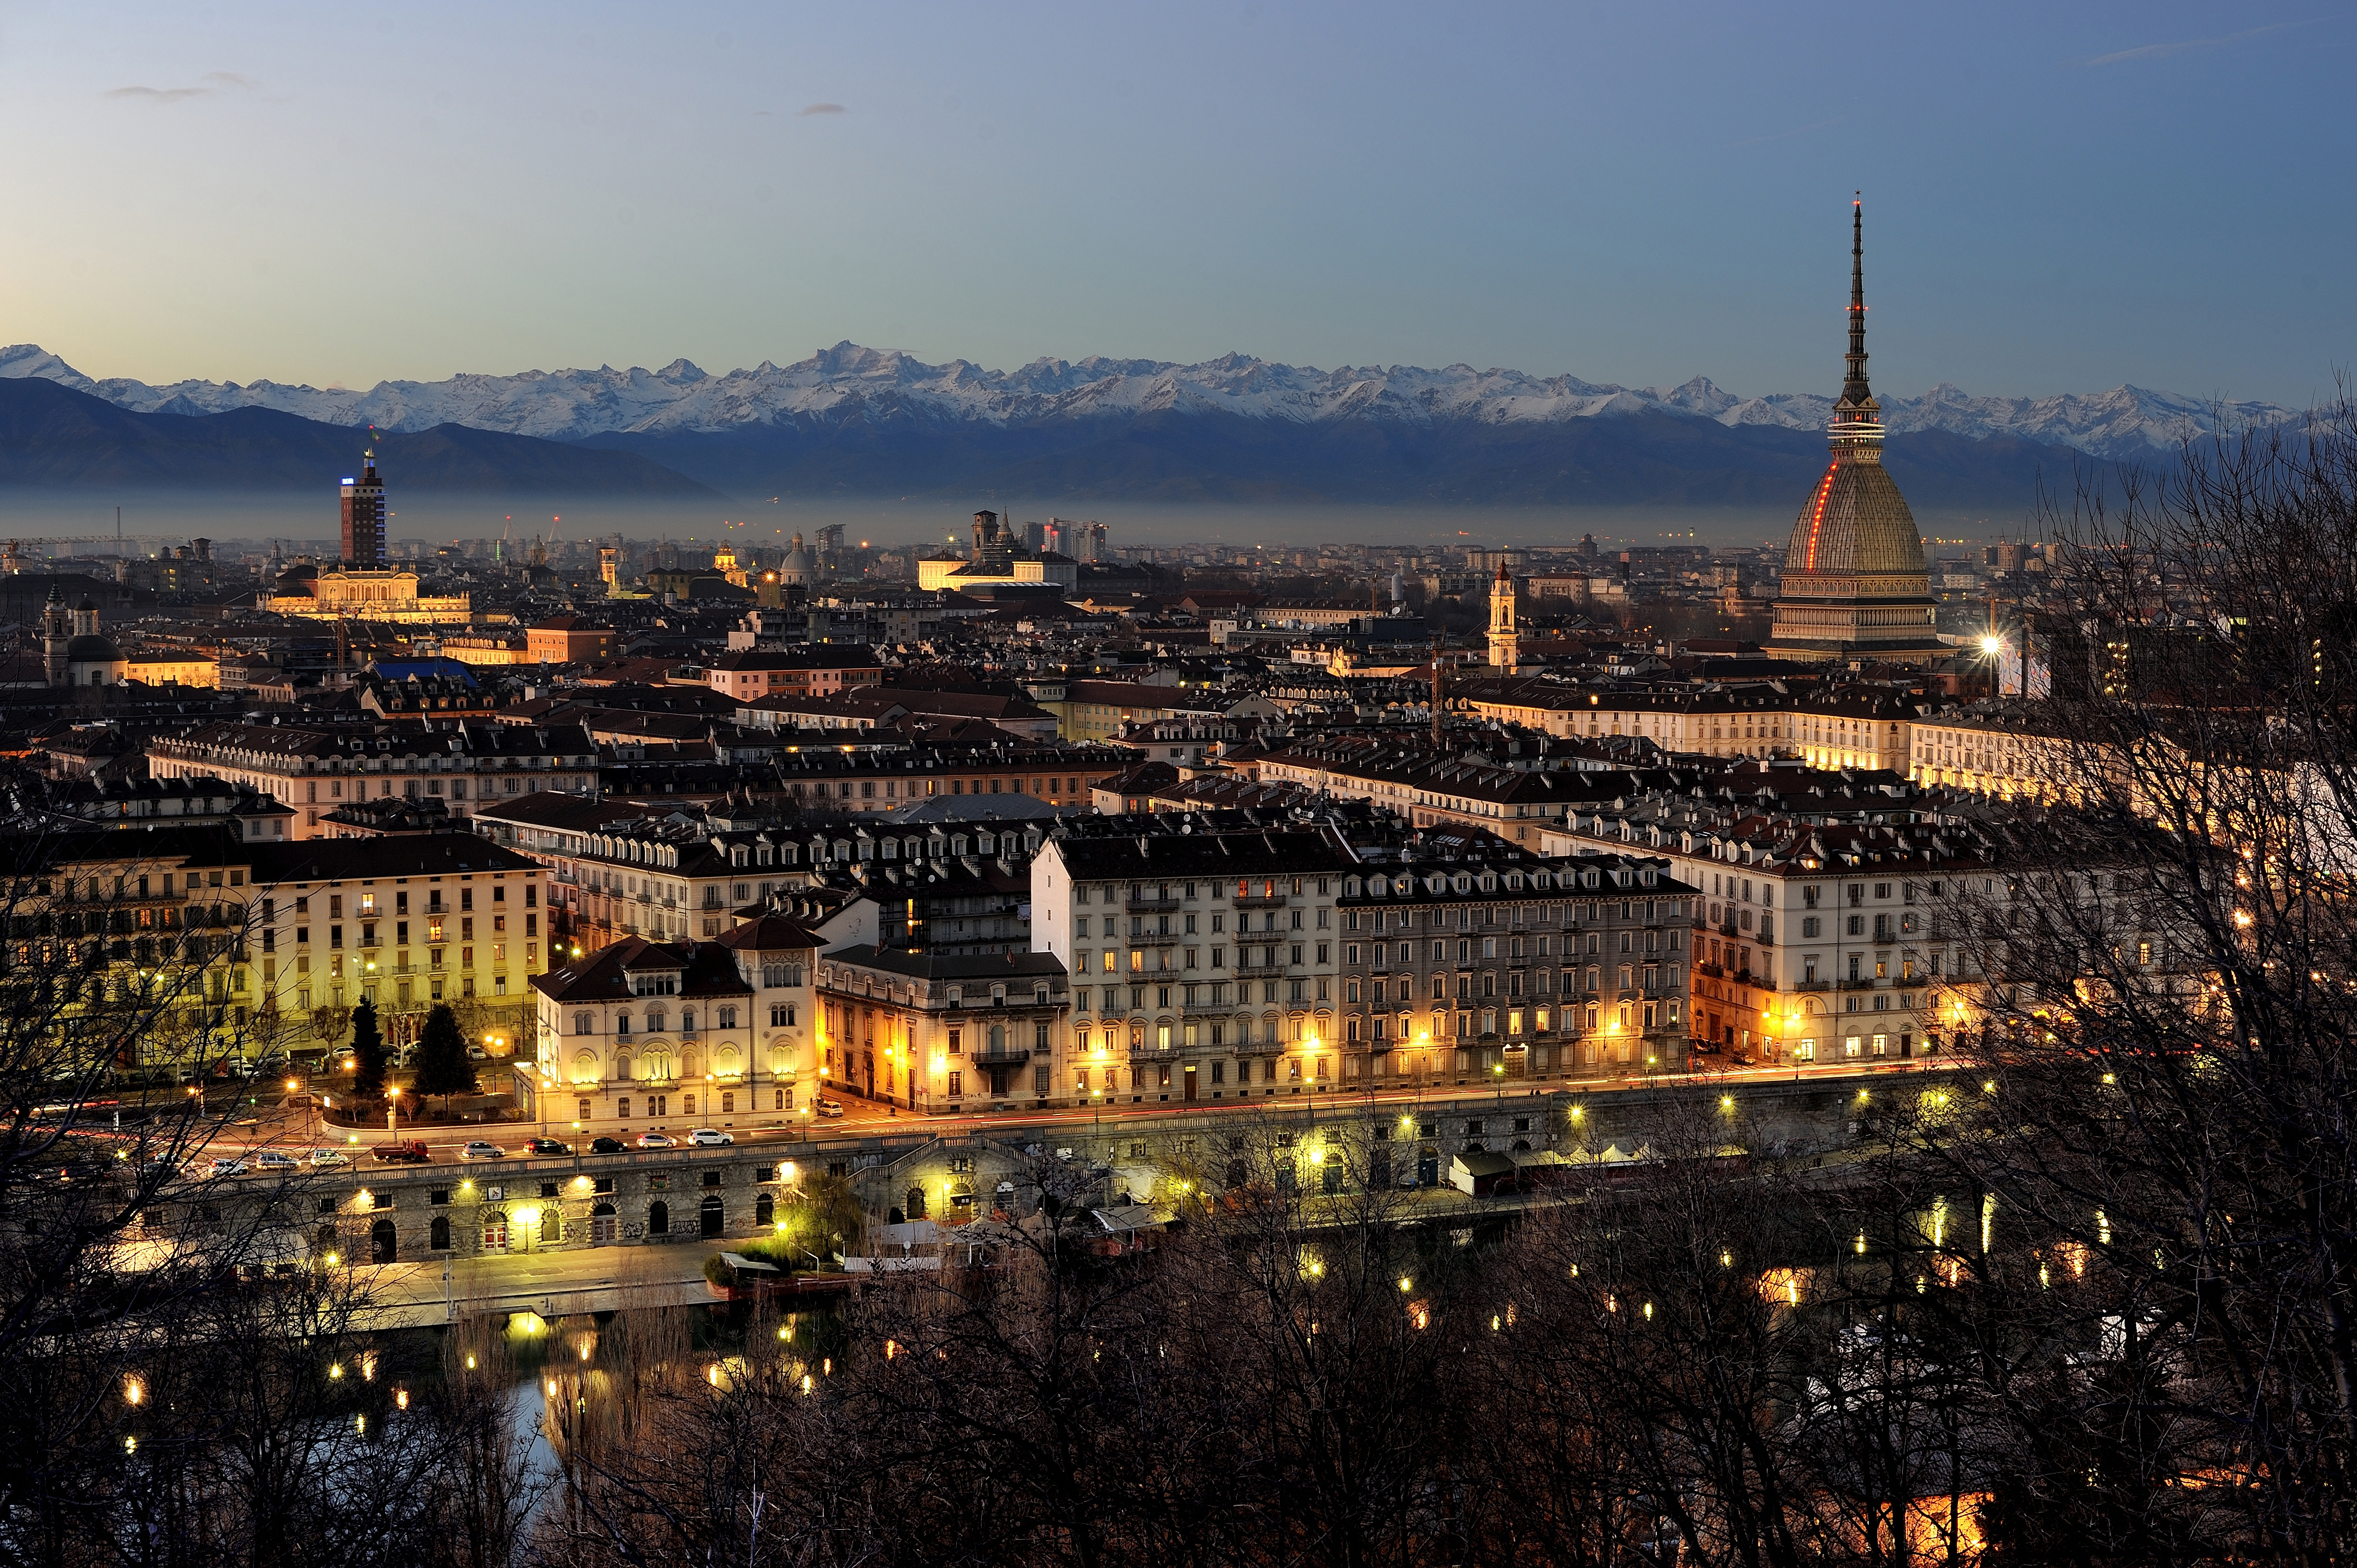
\includegraphics[width=10cm]{files/Turin_monte_cappuccini.jpg}
    \caption{Immagine referenziata dal link ricevuto}
\end{figure}
\newpage
\subsection{Query di utilità}
Presentiamo ora delle query che usiamo nell'applicazione client per completare le query precedentemente mostrate. Queste query di utilità sono molto semplici ma essenziali e ci è parso opportuno riportarle anche nella documentazione.\newline
Per ottenere tutte le città presenti nell'ontologia:
\begin{lstlisting}[language=SPARQL]
PREFIX deliverydr: 
<http://www.semanticweb.org/progettomodsem2020/deliverydoctor#>

SELECT ?nome
WHERE {
    ?c a deliverydr:Citta;
       deliverydr:haNome ?nome
}
ORDER BY ?nome
\end{lstlisting}
\begin{tabularx}{\textwidth} { 
  | >{\centering\arraybackslash}X |}
 \hline
 \textbf{?nome} \\
 \hline
 \textit{Asti} \\
 \hline
 \textit{Avigliana} \\
 \hline
 \textit{Mondovì} \\
 \hline
 \textit{Torino} \\
\hline
\end{tabularx}
\newline
\newline
Per ottenere tutti i nomi delle persone presenti nell'ontologia:
\begin{lstlisting}[language=SPARQL]
PREFIX deliverydr: 
<http://www.semanticweb.org/progettomodsem2020/deliverydoctor#>

SELECT ?nome
WHERE {
    ?p a deliverydr:Persona;
       deliverydr:haNome ?nome
}
ORDER BY ?nome
\end{lstlisting}
\begin{tabularx}{\textwidth} { 
  | >{\centering\arraybackslash}X |}
 \hline
 \textbf{?nome} \\
 \hline
 \textit{Federico Torrielli} \\
 \hline
 \textit{Gianni} \\
 \hline
 \textit{Ivan Spada} \\
 \hline
 \textit{Luca} \\
 \hline
 \textit{Stefano Vittorio Porta} \\
 \hline
 \textit{Lorenzo Sciandra} \\
\hline
\end{tabularx}
\newline
\newline
Per ottenere i nomi di tutti i locali presenti:
\begin{lstlisting}[language=SPARQL]
PREFIX deliverydr: 
<http://www.semanticweb.org/progettomodsem2020/deliverydoctor#>

SELECT ?nomeLocale
WHERE {
    ?locale a deliverydr:EsercizioAlimentare;
            deliverydr:haNome ?nomeLocale.
}
ORDER BY ?nomeLocale
\end{lstlisting}
\begin{tabularx}{\textwidth} { 
  | >{\centering\arraybackslash}X |}
 \hline
 \textbf{?nome} \\
 \hline
 \textit{Dubai Coffee Lounge} \\
 \hline
 \textit{Galaxy Burger} \\
 \hline
 \textit{Napples} \\
 \hline
 \textit{Kingyo} \\
 \hline
 \textit{Noir Caffè} \\
\hline
\end{tabularx}
\newline
\newline

Infine, per ottenere i nomi di tutti gli ingredienti inseriti nell'ontologia:
\begin{lstlisting}[language=SPARQL]
PREFIX skos: <http://www.w3.org/2004/02/skos/core#>
PREFIX deliverydr: 
<http://www.semanticweb.org/progettomodsem2020/deliverydoctor#>

SELECT ?nome
WHERE {
    ?i a deliverydr:ingrediente;
       skos:prefLabel ?nome.
    FILTER ( lang(?nome) = "it" )
}
ORDER BY ?nome
\end{lstlisting}
\begin{tabularx}{\textwidth} { 
  | >{\centering\arraybackslash}X |}
 \hline
 \textbf{?nome} \\
 \hline
 \textit{Aceto di Vino Bianco} \\
 \hline
 \textit{Acido tartarico} \\
 \hline
 \textit{Acqua} \\
 \hline
 \textit{Albicocca} \\
 \hline
 ... \\
\hline
\end{tabularx}

\newpage
\section{Applicazione Client}
Il client è stato realizzato usando HTML5, Bootstrap 5, Vue.js e JQuery. Per la grafica abbiamo preso ispirazione dai \hyperref[sec:mockupFinali]{figure 1 e 2} in cui immaginavamo un mockup dell'ipotetica applicazione finale.
\newline
Il client si presenta quindi con una prima pagina html dedicata allo smistamento verso le 4 pagine che daranno la possibilità di eseguire le query introdotte nella selezione precedente, suddivise in base all'utente. 
% https://tex.stackexchange.com/a/16584/232428
\begin{figure}[H]
    \makebox[\textwidth][c]{\includegraphics[width=15cm]{files/index.png}}
    \caption{Pagina iniziale del client}
\end{figure}
Prendendo come esempio la sezione dell'utente normale, la nuova pagina presenterà una selezione tra le 3 queries introdotte.
\begin{figure}[H]
    \makebox[\textwidth][c]{\includegraphics[width=15cm]{files/utenteNormale.png}}
    \caption{Pagina per eseguire le query di un utente normale}
\end{figure}
Come è possibile vedere, la pagina presenta due dropdown:
\begin{itemize}
    \item Una prima, statica, dedicata alla scelta della query che si desidera effettuare tra quelle pre-impostate
    \item Una seconda, dinamica, i cui valori sono ottenuti con una richiesta http asincrona indirizzata al server GraphDB. Una volta recuperati, i valori permettono di completare la query scelta nella prima dropdown e di eseguirla.
\end{itemize}
Nel caso in cui non fosse selezionato nessun parametro nella seconda select, avremmo la situazione presentata in figura. Mostriamo ora un risultato totale di una query.
\begin{figure}[H]
    \makebox[\textwidth][c]{\includegraphics[width=15cm]{files/utenteNormale2.png}}
    \caption{Risultati della query di ricerca di locali con pietanze senza glutine a Torino}
\end{figure}
Una volta scelto un valore per entrambe le dropdown, Vue si accorgerà di questo cambiamento ed eseguirà automaticamente la query. I risultati vengono richiesti al server GraphDB in formato CSV e, una volta ricevuti, saranno prima parsificati e successivamente inseriti in una tabella costruita dinamicamente grazie a Vue.js.
\section{Regole SWRL}
In questa sezione sarà presentata la base delle regole SWRL usate nel progetto. Vediamo come prime regole quelle che riguardano i ruoli assunti dalle persone. Le 4 regole che abbiamo usato per definire correttamente il ruolo di una persona si basano sulle seguenti considerazioni:
\begin{itemize}
    \item se una persona ha eseguito almeno un ordine le verrà inferito il ruolo Ruolo Cliente;
    \item se un individuo ha recensito almeno un locale allora avrà associato il Ruolo Recensore;
    \item se una persona ha consegnato almeno un ordine avrà il Ruolo Fattorino;
    \item se un individuo ha avviato almeno un'impresa allora avrà il Ruolo Titolare.
\end{itemize}
\begin{lstlisting}[language=SPARQL]
    RuoloCliente(?x) ^ ordinatoDa(?y, ?z) -> haRuolo(?z, ?x)
    
    RuoloFattorino(?x) ^ consegnatoDa(?y, ?z) -> haRuolo(?z, ?x)
    
    RuoloRecensore(?x) ^ recensitoDa(?y, ?z) -> haRuolo(?z, ?x)
    
    RuoloTitolareImpresa(?x) ^ impresaAvviataDa(?y, ?z) -> 
                                                        haRuolo(?z, ?x)
\end{lstlisting}
Passiamo ora alla regola SWRL che classifica un locale come Esercizio Alimentare Non Ottimo nel momento in cui questo abbia associato anche una sola recensione con una stella.
\begin{lstlisting}[language=SPARQL]
    recensioneCreataDaAzione(?x, ?y) ^ recensireLocale(?y, ?z) ^
    schema:reviewRating(?x, ?s) ^ possiedeStelle(?s, ?c) ^
    swrlb:equal(?c, 1) -> EsercizioAlimentareNonOttimo(?z)
\end{lstlisting}
Mostriamo ora le 2 regole usate per classificare le pietanze in base al numero di ingredienti di cui necessitano. Classificheremo una pietanza come semplice nel caso in cui richiedesse al più 3 ingredienti, mentre sarà considerata complessa nel momento in cui necessitasse di almeno 10.
\begin{lstlisting}[language=SPARQL]
    Pietanza(?x) ^ haNumeroIngredienti(?x, ?n) ^ 
            swrlb:lessThanOrEqual(?n, 3) -> PietanzaSemplice(?x)
    
    Pietanza(?x) ^ haNumeroIngredienti(?x, ?n) ^ 
           swrlb:greaterThanOrEqual(?n, 10) -> PietanzaComplessa(?x)
\end{lstlisting}
\newpage
Concludiamo con 2 regole che permettono di inferire il fatto che un locale sia situato in una determinata città a partire dal fatto che sia situato in una sua via, o in una sua piazza.
\begin{lstlisting}[language=SPARQL]
    localeSituatoIn(?x, ?y) ^ Via(?y) ^ viaDellaCitta(?y, ?z) ->
                                                localeSituatoIn(?x, ?z)
    
    localeSituatoIn(?x, ?y) ^ Piazza(?y) ^ piazzaDellaCitta(?y, ?z)
                                            -> localeSituatoIn(?x, ?z)
\end{lstlisting}
\section{Allegati Full Size}
Saranno presentate, in questa sezione finale della documentazione, alcune delle immagini ingrandite inserite nelle sezioni precedenti che a causa dello spazio limitato potevano risultare di difficile lettura.
    \incgraph[graphicspaper]{files/gerarchia.png}
\end{document}